% \documentclass[draft]{beamer}
\documentclass{beamer}
% 20181219
% 20190311
% 20190312
% 20190313
% 20190314

% 20190315 v1
% 20191108 v1.1

\usepackage{indentfirst}
	\setlength{\parindent}{2em}
\usepackage{changepage}
\usepackage{calc}
\usepackage{mdwlist}

\usepackage{ctex}
\usepackage{xeCJK}
	\xeCJKsetup{CJKecglue={\hskip 0pt plus 0pt}}

\usepackage{ulem}
\usepackage{marvosym}
\usepackage{perpage}
	\MakePerPage{footnote}

\usepackage{beamerthemesplit}  
	\setbeamersize{text margin left=3em, text margin right=3em}
	\setbeamertemplate{description item}[align right] % 20171011 
	\addtobeamertemplate{navigation symbols}{}{%
		\usebeamerfont{footline}%
		\usebeamercolor[fg]{footline}%
		\hspace{1em}%
		\insertframenumber/\inserttotalframenumber
	}
	\setbeamertemplate{itemize items}{\textbf{\texttt{>\hskip-.2em-\hskip-.2em-}}}
	% 20191108
	\makeatletter
	\let\old@beamer@@frametitle\beamer@@frametitle
	\def\beamer@@frametitle[#1]#2{\old@beamer@@frametitle[#1]{\qquad #2}}
	\makeatother

\usepackage{ruby}
	\renewcommand{\rubysize}{0.8}
	\renewcommand{\rubysep}{0ex}

\usepackage{graphicx}

\title{正则表达式简介}
\author[杨宇昌]{杨宇昌%
	\begingroup\def\thefootnote{\Letter}%
	\rlap{\,\footnote{\,\texttt{yang.yc.allium@gmail.com}}}%
	\endgroup}
\institute{\small 中国科学院植物研究所\\系统与进化植物学国家重点实验室}
\date{2019 年 11 月 8 日\qquad ver 1.1}

\usepackage{color}
	\definecolor{miku}{RGB}{57, 197, 187}
	\definecolor{beamer@blendedblue}{RGB}{19, 149, 139}
	\definecolor{mikudark}{RGB}{19, 149, 139}
	\definecolor{mikuribbon}{RGB}{228, 0, 127}
	\def\mymikudark#1{{\color{beamer@blendedblue}#1}}
	\def\mymikuribbon#1{{\color{mikuribbon}#1}}

\usepackage{fancyvrb}
	\fvset{formatcom=\color{mikuribbon},showspaces=true,codes={\catcode`$=3}}
	\DefineShortVerb{\!}
	\renewcommand{\theFancyVerbLine}{\footnotesize\arabic{FancyVerbLine}}
	\DefineVerbatimEnvironment{YVerb}{Verbatim}{%
		numbers=left,frame=single,numbersep=1ex,%
		gobble=9,formatcom=\color{mikudark}}
	\newcommand{\txt}[1]{\mymikudark{\texttt{#1}}}
	% 20191108
	\let\FancyVerbSpace\textvisiblespace

\def\replace{{\color{black} $\Rightarrow$ }}
\def\showspace{\makebox[0.5em][c]{$\cdot$}}
\def\showtab{\makebox[2em][c]{\ensuremath{\longrightarrow}}}
\def\nothing{\mymikuribbon{$\varnothing$}}
\def\intagliated#1{\hskip0.05em\raisebox{-0.15em}{{\ooalign{%
	\rule{1em}{1em}\cr
	\hidewidth{\raisebox{0.165em}{\color{white}\scalebox{0.7}[1]{#1}}}\hidewidth\cr}%
	}}\hskip0.05em
}
\def\showCR{\intagliated{CR}}
\def\showLF{\intagliated{LF}}

\def\npp{Notepad++}
\def\source{Source}
\def\target{Target}

\newenvironment{igsimple}%
	{\begin{description*}\leftskip=-3em\relax\item[例:\kern-1ex]}%
	{\end{description*}}

\newlength{\relaxlen}
\setlength{\relaxlen}{.1em}
\newcommand\pnoun[1]{\hskip\relaxlen\underline{\kern-\relaxlen\hbox{#1\kern-\relaxlen}}\hskip\relaxlen} % 20181226

\usepackage{bookmark}
\usepackage{etoolbox}
\newif\ifprintbookmark
\printbookmarktrue
\makeatletter
\newcommand{\bookm}[2]{\bookmark[page=\the\c@page,level=#1]{#2}}
\apptocmd{\beamer@@frametitle}{\ifprintbookmark\only<1>{\bookmark[page=\the\c@page,level=4]{#1}}\fi}%
{\message{** patching of \string\beamer@@frametitle succeeded **}}%
{\message{** patching of \string\beamer@@frametitle failed **}}%
\makeatother

%%%%%%%%%%%%%%%%%%%%%%%%%%%%%%%%%%%%%%%%%%%%%%%%%%%%%%%%%%%%%%%%

\begin{document}

\parskip=1ex
\parindent=0.1em

\bookm{2}{封面}

\frame{\titlepage}

\printbookmarkfalse

\bookm{2}{使用许可协议}
\begin{frame}{使用许可协议}
	本文档依 CC BY-NC-SA 4.0 协议\footnote{\texttt{https://creativecommons.org/licenses/by-nc-sa/4.0/deed.zh}}授权\hfill
	\parbox[c]{3cm}{\includegraphics[width=3cm]{Illustratio/CC_BY-NC-SA.eps}}\par
	只要遵守以下条件,即可自由地共享和演绎本作品:
	\begin{itemize}\leftskip=2em
		\item 署名(BY)
		\item 非商业性使用(NC)
		\item 相同方式共享(SA)
	\end{itemize}
	\medskip
	本文档的源代码见
	\centerline{\strut\color{mikudark}\texttt{https://github.com/Mikumikunisiteageru/RegEx\_Lecture}}
\end{frame}

\bookm{2}{目录}
\begin{frame}{目录}
	\parskip=0em
	\parindent=2em
	\tableofcontents
\end{frame}

\AtBeginSection[]{
	\printbookmarkfalse
	\begin{frame}{目录}
		\parskip=0em
		\parindent=2em
		\tableofcontents[currentsection]
	\end{frame}
	\printbookmarktrue
	\parskip=1ex
}

\printbookmarktrue

\section{绪论}

\subsection{正则表达式}

\begin{frame}[fragile]{进阶查找与替换:正则表达式}
	正则表达式 / Regular Expression:按照规则匹配模式\par
	推荐软件:\npp\footnote{\texttt{https://notepad-plus-plus.org/}},使用的正则表达式流派为 PCRE\footnote{\texttt{http://docs.notepad-plus-plus.org/index.php/Regular\_Expressions}}\par
	本幻灯片记号约定
	\begin{itemize}
		\item \txt{这样的文字} 或 \txt{such text} 表示实际的文本
		\item !这样的文字! 或 !such text! 表示正则表达式
		\item !查找目标Source! \replace !替换为Target! 表示一次替换操作
	\end{itemize}\par
\end{frame}

\subsection{中文编码问题}

\begin{frame}[fragile]{中文编码:ANSI 与 UTF-8}
	在“格式”菜单中,可以检查当前文本文件的编码
	\def\rubysize{0.4}
	\begin{itemize}
		\item ANSI 是坏编码,不能抵抗字节丢失,容错性低\\
			\def\rubysep{-0.2ex}
			\pnoun{TGC}\pnoun{ATG}\pnoun{CCT}\pnoun{GCA}…~$\rightarrow$ \pnoun{GCA}\pnoun{TGC}\pnoun{CTG}CA…\\
			\vskip1ex
			\txt{\ruby{且}{\,C7\;D2\,}\ruby{持}{\,B3\;D6\,}\ruby{梦}{\,C3\;CE\,}\ruby{笔}{\,B1\;CA\,}\ruby{书}{\,CA\;E9\,}\ruby{奇}{\,C6\;E6\,}\ruby{景}{\,BE\;B0\,}} $\rightarrow$ \txt{\ruby{页}{\,D2\;B3\,}\ruby{置}{\,D6\;C3\,}\ruby{伪}{\,CE\;B1\,}\ruby{适}{\,CA\;CA\,}\ruby{槠}{\,E9\;C6\,}\ruby{婢}{\,E6\;BE\,}\ruby{?}{\,B0\,}}
		\item UTF-8 是好编码,有分组机制,局部错误不会扩散\\
			\def\rubysep{-0ex}
			TGC ATG CCT GCA…~$\rightarrow$ GC ATG CCT GCA…\\
			\vskip1ex
			\txt{\ruby{日}{\,E6\;97\;A5\,}\ruby{破}{\,E7\;A0\;B4\,}\ruby{云}{\,E4\;BA\;91\,}\ruby{波}{\,E6\;B3\;A2\,}\ruby{万}{\,E4\;B8\;87\,}\ruby{里}{\,E9\;87\;8C\,}\ruby{红}{\,E7\;BA\;A2\,}} $\rightarrow$ \txt{\ruby{??}{\,97\;A5\,}\ruby{破}{\,E7\;A0\;B4\,}\ruby{云}{\,E4\;BA\;91\,}\ruby{波}{\,E6\;B3\;A2\,}\ruby{万}{\,E4\;B8\;87\,}\ruby{里}{\,E9\;87\;8C\,}\ruby{红}{\,E7\;BA\;A2\,}} 
	\end{itemize}
	执行查找或替换操作前,必须确认编码方式为 UTF-8
\end{frame}

\subsection{不可见字符}

\begin{frame}[fragile]{观察不可见字符}
	按第七组第二个按钮 $\P$\footnote{或“视图”——“显示符号”——“显示所有字符”} 可以看到平时不可见的字符
	\begin{itemize}
		\item 空格,按 Spacebar 键输入,记作 ! !,显示为 \txt{\showspace}\\
			!space between words! $\Leftrightarrow$ \txt{space\showspace between\showspace words}
		\item 全角空格,在中文输入法全角状态下按 Spacebar 键输入
		\item 制表符,按 Tab 键输入,记作 !\t!,显示为 \txt{\showtab}\\
			\txt{\showtab} 随位置不同可长可短,但都同样是一个制表符
		\item 换行符,按 Enter 键输入,记作 !\r\n!,显示为 \txt{\showCR \showLF}\\
			Windows 风格的换行是 !\r\n!,其他操作系统的是 !\n!
	\end{itemize}\par
	用正则表达式替换时,最好打开 $\P$ 开关,以便观察效果
\end{frame}

\begin{frame}[fragile]{制表符的作用}
	制表符常用于与电子表格软件\footnote{如 Microsoft Excel}联合作业\par
	\only<1>{电子表格复制到纯文本环境时,列用 \mymikuribbon{\textbackslash t} 分隔,即 TSV 格式\par}
	\only<2>{TSV 复制到电子表格时,\mymikuribbon{\textbackslash t} 分隔列,不带字体风格\par}
	\vskip1em
	\parindent=0em
	\only<1>{\begin{minipage}[c]{25.5ex}
		\begin{tabular}{|l|l|}
			\hline
			\textbf{中文名} & \textbf{学名} \\\hline
			南蝠 & \textit{Ia io} Thomas\\\hline
			大蟾蜍 & \textit{Bufo bufo} L.\\\hline
			喜鹊 & \textit{Pica pica} L.\\\hline
			翻车鱼 & \textit{Mola mola} L.\\\hline
			玉蜀黍 & \textit{Zea mays} L.\\\hline
			早熟禾 & \textit{Poa annua} L.\\\hline
		\end{tabular}
		\par\vbox to 0.4em{}
	\end{minipage}}
	\only<2>{\begin{minipage}[c]{25.5ex}
		\begin{tabular}{|l|l|}
			\hline
			中文名 & 学名 \\\hline
			南蝠 & {Ia io} Thomas\\\hline
			大蟾蜍 & {Bufo bufo} L.\\\hline
			喜鹊 & {Pica pica} L.\\\hline
			翻车鱼 & {Mola mola} L.\\\hline
			玉蜀黍 & {Zea mays} L.\\\hline
			早熟禾 & {Poa annua} L.\\\hline
		\end{tabular}
		\par\vbox to 0.4em{}
	\end{minipage}}
	\hfill\only<1>{$\Rightarrow$}\only<2>{$\Leftarrow$}\quad\hfill
	\begin{minipage}[c]{27.5ex}
		\def\@{\showtab}
		\begin{YVerb}[commandchars=\\\{\}]
			中文名\@学名
			南蝠\@Ia io Thomas
			大蟾蜍\@Bufo bufo L.
			喜鹊\@Pica pica L.
			翻车鱼\@Mola mola L.
			玉蜀黍\@Zea mays L.
			早熟禾\@Poa annua L.
		\end{YVerb}
	\end{minipage}\par
\end{frame}

%%%%%%%%%%%%%%%%%%%%%%%%%%%%%%%%%%%%%%%%%%%%%%%%%%%%%%%%%%%%%%%%

\section{语法}

\subsection{转义}

\begin{frame}[fragile]{特殊字符的转义}
	正则表达式中,以下 14 个字符是特殊的,不能直接表示\par
	\hfill\txt{* . ? + \$ \string^ [ ] ( ) \{ \} | \string\ }\hfill\hbox{}\par
	要表示这些字符,需要在前面加上反斜线 !\!\par
	例:!\*! 表示 \txt{*},!\.! 表示 \txt{.},!\\! 表示 \txt{\textbackslash}\par
	特殊字符在正则表达式中承担语法功能,如 !.! 匹配任何字符\par
	\begin{igsimple}
		!3.14! 可匹配 \txt{3.14}、\txt{3014}、\txt{3d14} 或 \txt{3点14}\\
		!3\.14! 只可匹配 \txt{3.14}
	\end{igsimple}
\end{frame}

\subsection{集合、量词与分组}

\begin{frame}[fragile]{集合与通配符}
	\begin{itemize}
		\item ![…]! 正集合,匹配其中任何字符
		\item ![^…]! 负集合,匹配其外任何字符,慎用
		\item !.! 匹配任意字符(除了 !\r! 与 !\n!\footnote{关闭“\mymikuribbon{\texttt{.}} 匹配新行”的选项即可如此})
		\item !\d! 匹配阿拉伯数字,等价于 ![0-9]!
		\item !\l! 匹配小写罗马字母,等价于 ![a-z]!
		\item !\u! 匹配大写罗马字母,等价于 ![A-Z]!
		\item ![\x{3400}-\x{9FFF}]! 匹配中日韩汉字
	\end{itemize}
	\begin{igsimple}
		![一二三]球悬铃木! 可匹配 \txt{一球悬铃木}~或 \txt{三球悬铃木}\\
		!201\d! 可匹配 \txt{2010} 或 \txt{2019}
	\end{igsimple}
\end{frame}

\begin{frame}[fragile]{量词}
	量词表示其前面的模式重复的次数,不可单独使用\par
	\begin{itemize}
		\item !{$a$,$b$}! 至少 $a$ 次,至多 $b$ 次\footnote{$a$ 与 $b$ 均为非负整数,且 $a\leq b$,下同}
		\item !{$a$,}! 至少 $a$ 次,无上限
		\item !{$a$}! 恰好 $a$ 次,等价于 !{$a$,$a$}!
		\item !+! 至少 1 次,无上限,等价于 !{1,}!
		\item !*! 至少 0 次,无上限,等价于 !{0,}!
		\item !?! 至少 0 次,至多 1 次,等价于 !{0,1}!
	\end{itemize}
	\vspace*{-0.5em}
	\begin{igsimple}
		!nat?ive! 可匹配 \txt{naive} 或 \txt{native}\par
		!em+! 可匹配 \txt{em} 或 \txt{emmmmmm},但不可匹配 \txt{e}\par
		!\d{4}! 可匹配 \txt{2019},也可匹配 \txt{6666}
	\end{igsimple}
\end{frame}

\begin{frame}[fragile]{量词的贪婪性}
	量词默认是贪婪的,即匹配尽可能长的字符串
	\begin{igsimple}
		字符串 \txt{20190831} 中, \\
		!\d{4,8}! 倾向于匹配 \txt{20190831} 而不是 \txt{2019}
	\end{igsimple}\par
	要抑制贪婪,需要在量词后添加 !?!
	\begin{igsimple}
		字符串 \texttt{20190831} 中, \\
		!\d{4,8}?! 倾向于匹配 \txt{2019} 而不是 \txt{20190831}
	\end{igsimple}
	注意:!*?! 和 !??! 都是合法的,但没得必要
\end{frame}

\begin{frame}[fragile]{分组与捕捉}
	圆括号 !(…)! 可以把模式分组,形成更长的模式
	\begin{igsimple}
		!(\d+.){2}! 可以匹配 \txt{1年365天} 或 \txt{10下10下}
	\end{igsimple}\par
	分组按照开始的顺序,分别自动命名为 !\1!、!\2!、!\3! 等
	\begin{igsimple}
		!(.)(.)\1\2! 可匹配 \txt{开心开心},不可匹配 \txt{开开心心} \\
		!(.)\1(.)\2! 可匹配 \txt{开开心心},不可匹配 \txt{开心开心}
	\end{igsimple}
	分组在替换中仍然有效,可以 !\1!、!\2! 等方式引用
	\begin{igsimple}
		要把碱基序列 \txt{TGCATGCCTGCA} 每三个字母用空格分隔,\\
		作替换 !(\u{3})! \replace !\1 ! 即可得到 \txt{TGC ATG CCT GCA }
	\end{igsimple}
\end{frame}

\fvset{codes={}}

\subsection{位置与或运算}

\begin{frame}[fragile]{锚点}
	锚点匹配位置,没有宽度
	\begin{itemize}
		\item !^! 行开始处(\texttt{\string\r\string\n} 之后或文档开始处)
		\item !$! 行结束处(\texttt{\string\r\string\n} 之前或文档结束处)
		\item !\<! 单词\footnote{\;中文无词式书写习惯,不适用于 Scintilla 准则,故无单词一说}开始处
		\item !\>! 单词结束处
		\item !\b! 单词边界处
	\end{itemize}
	\vspace*{-0.5em}
	\begin{igsimple}
		\txt{The \uline{car} is s\uline{car}let} 中,\\
		!car! 有两处匹配,!\<car\>! 或 !\bcar\b! 只匹配前一处\par
	\end{igsimple}
\end{frame}

\begin{frame}[fragile]{例:去除空行}
	\parindent=0em
	\hbox{}\hfill
	\begin{minipage}[c]{12.5ex}
		\begin{YVerb}[label=\source]
			Non-empty

			Non-empty

			Non-empty


			Non-empty
		\end{YVerb}
	\end{minipage}%
	\hfill
	\begin{minipage}[c]{20ex}
		\centering
		!^\r\n! \replace \nothing\footnotemark[1]\par
		或\par
		!(\r\n){2,}! \replace !\1!
	\end{minipage}\quad%
	\hfill
	\begin{minipage}[c]{12.5ex}
		\begin{YVerb}[label=\target]
			Non-empty
			Non-empty
			Non-empty
			Non-empty
		\end{YVerb}
	\end{minipage}
	\hfill\hbox{}\footnotetext{替换为空白,相当于删除匹配到的模式,后同}\par
\end{frame}

\begin{frame}[fragile]{例:去除前导零}
	\parindent=0em
	\hbox{}\hfill
	\begin{minipage}[c]{12.5ex}
		\begin{YVerb}[label=\source]
			000076962
			00165087
			00247904
			00386584
			000844259
			00034441
			00034449
			1217872
		\end{YVerb}
	\end{minipage}%
	\hfill
	\begin{minipage}[c]{11ex}
		!^0+! \replace \nothing
	\end{minipage}%
	\hfill
	\begin{minipage}[c]{10.5ex}
		\begin{YVerb}[label=\target]
			76962
			165087
			247904
			386584
			844259
			34441
			34449
			1217872
		\end{YVerb}
	\end{minipage}
	\hfill\hbox{}\par
\end{frame}

\begin{frame}[fragile]{例:添加前导零}
	\parindent=0em
	\hbox{}\hfill
	\begin{minipage}[c]{10.5ex}
		\begin{YVerb}[label=\source]
			76962
			165087
			247904
			386584
			844259
			34441
			34449
			1217872
		\end{YVerb}
	\end{minipage}%
	\hfill
	\begin{minipage}[c]{28ex}
		\begin{enumerate}
			\item !^(\d{1,7})$! \replace !0\1!
			\item 重复 1 至匹配不到
		\end{enumerate}
	\end{minipage}%
	\hfill
	\begin{minipage}[c]{11.5ex}
		\begin{YVerb}[label=\target]
			00076962
			00165087
			00247904
			00386584
			00844259
			00034441
			00034449
			01217872
		\end{YVerb}
	\end{minipage}
	\hfill\hbox{}\par
\end{frame}

\begin{frame}[fragile]{零宽断言}
	\UndefineShortVerb{\!}
	\DefineShortVerb{\+}
	零宽断言匹配位置,也没有长度
	\begin{itemize}
		\item +(?=…)+ 后面会有该模式
		\item +(?!…)+ 后面不会有该模式
		\item +(?<=…)+ 前面有了该模式
		\item +(?<!…)+ 前面没有该模式
	\end{itemize}
	\begin{igsimple}
		+(?<=\d)km\>+ \replace + km+ 可以把 \txt{3km} 更正为 \txt{3 km}
	\end{igsimple}
	注意:用负断言(+(?!…)+ 或 +(?<!…)+)时要小心
	\UndefineShortVerb{\+}
	\DefineShortVerb{\!}
\end{frame}

\begin{frame}[fragile]{例:用下划线分隔馆代号与标本号}
	\parindent=0em
	\hbox{}\hfill
	\begin{minipage}[c]{15.5ex}
		\begin{YVerb}[label=\source]
			BM000076962
			G00165087
			NY00247904
			E00386584
			K000844259
			PE00034441
			PE00034449
			KUN1217872
		\end{YVerb}
	\end{minipage}%
	\hfill
	\begin{minipage}[c]{27ex}
		\centering
		!(?<=\u)(?=\d)! \replace !_!\par
		或\par
		!(\u)(\d)! \replace !\1_\2!
	\end{minipage}\quad%
	\hfill
	\begin{minipage}[c]{16.5ex}
		\begin{YVerb}[label=\target]
			BM_000076962
			G_00165087
			NY_00247904
			E_00386584
			K_000844259
			PE_00034441
			PE_00034449
			KUN_1217872
		\end{YVerb}
	\end{minipage}%
	\hfill\hbox{}\par
\end{frame}

\begin{frame}[fragile]{大小写转换}
	\npp{} 提供了“匹配大小写”选项,平时建议开启\par
	\begin{igsimple}
		关闭该选项时,!\<mL\>! \replace !mL! 可将 \txt{ml}、\txt{ML} 等统一为 \txt{mL}
	\end{igsimple}
	强制罗马字母大小写
	\begin{itemize}
		\item !\u! 其后一个字母强制大写
		\item !\U…\E! 其间全部字母强制大写
		\item !\l! 其后一个字母强制小写
		\item !\L…\E! 其间全部字母强制小写
	\end{itemize}\par
	\begin{igsimple}
		!\<(\l)! \replace !\u\1! 可将所有单词首字母大写,用于书名
	\end{igsimple}
\end{frame}

\begin{frame}[fragile]{或运算}
	!…|…! 可匹配前面的或后面的模式,其优先级低于连接运算\par
	\begin{igsimple}
		!a (truck|lorry)! 可匹配 \txt{a truck} 或 \txt{a lorry}\par
		!a truck|lorry! 可匹配 \txt{a truck} 或 \txt{lorry}
	\end{igsimple}\par
	正则表达式中的运算优先级
	$$\mbox{转义}>\mbox{分组、零宽断言与集合}>\mbox{量词}>\mbox{锚点与连接}>\mbox{或}$$
\end{frame}

%%%%%%%%%%%%%%%%%%%%%%%%%%%%%%%%%%%%%%%%%%%%%%%%%%%%%%%%%%%%%%%%

\section{例题}

\subsection{日期格式化}

\printbookmarkfalse
\bookm{4}{日期格式化:yyyy.m.d → yyyy.mm.dd}
\begin{frame}[fragile]{日期格式化:yyyy.m.d $\rightarrow$ yyyy.mm.dd}
	\begin{adjustwidth}{-0.5em}{-1.5em}
	\begin{minipage}[c]{13.5ex}
		\begin{YVerb}[label=\source]
			1559.2.21
			1592.11.28
			1638.3.15
			1654.5.4
			1678.12.13
			1711.11.25
			1760.11.13
			1782.9.16
			1831.7.17
			1856.4.27
			1871.8.14
			1906.2.7
		\end{YVerb}
	\end{minipage}
	\hfill
	\begin{minipage}[c]{\linewidth-30ex}
		\centering
		\begin{enumerate}
			\item !\.! \replace !\.0!
			\item !\.0?(\d\d)! \replace !\.\1!
		\end{enumerate}
		或\par
		!(?<=\.)(\d)(?=[\.\r])! \replace !0\1!
	\end{minipage}\quad
	\hfill
	\begin{minipage}[c]{13.5ex}
		\begin{YVerb}[label=\target]
			1559.02.21
			1592.11.28
			1638.03.15
			1654.05.04
			1678.12.13
			1711.11.25
			1760.11.13
			1782.09.16
			1831.07.17
			1856.04.27
			1871.08.14
			1906.02.07
		\end{YVerb}
	\end{minipage}
	\end{adjustwidth}
\end{frame}

\bookm{4}{日期格式化:yyyy.m.d → yyyymmdd}
\begin{frame}[fragile]{日期格式化:yyyy.m.d $\rightarrow$ yyyymmdd}
	\begin{minipage}[c]{13.5ex}
		\begin{YVerb}[label=\source]
			1559.2.21
			1592.11.28
			1638.3.15
			1654.5.4
			1678.12.13
			1711.11.25
			1760.11.13
			1782.9.16
			1831.7.17
			1856.4.27
			1871.8.14
			1906.2.7
		\end{YVerb}
	\end{minipage}
	\hfill
	\begin{minipage}[c]{27ex}
		\begin{enumerate}
			\item !\.! \replace !\.0!
			\item !\.0?(\d\d)! \replace !\1!
		\end{enumerate}
	\end{minipage}
	\hfill
	\begin{minipage}[c]{11.5ex}
		\begin{YVerb}[label=\target]
			15590221
			15921128
			16380315
			16540504
			16781213
			17111125
			17601113
			17820916
			18310717
			18560427
			18710814
			19060207
		\end{YVerb}
	\end{minipage}
\end{frame}

\bookm{4}{日期格式化:yyyymmdd → yyyy/m/d}
\begin{frame}[fragile]{日期格式化:yyyymmdd $\rightarrow$ yyyy/m/d}
	\begin{minipage}[c]{11.5ex}
		\begin{YVerb}[label=\source]
			15590221
			15921128
			16380315
			16540504
			16781213
			17111125
			17601113
			17820916
			18310717
			18560427
			18710814
			19060207
		\end{YVerb}
	\end{minipage}
	% \hfill
	\begin{minipage}[c]{\linewidth-30ex}
		\begin{enumerate}
			\item !(\d{4})(\d\d)(\d\d)! \replace !\1/\2/\3!
			\item !/0! \replace !/!
		\end{enumerate}
	\end{minipage}
	\hfill
	\begin{minipage}[c]{13.5ex}
		\begin{YVerb}[label=\target]
			1559/2/21
			1592/11/28
			1638/3/15
			1654/5/4
			1678/12/13
			1711/11/25
			1760/11/13
			1782/9/16
			1831/7/17
			1856/4/27
			1871/8/14
			1906/2/7
		\end{YVerb}
	\end{minipage}
\end{frame}

\subsection{动物的分类法}

\printbookmarktrue
\begin{frame}[fragile]{把动物按脚的数目分类}
	\vspace*{0.3em}
	\hfill
	\begin{minipage}[c]{15.5ex}
		\begin{YVerb}[label=\source]
			人有两只脚
			海星有五只脚
			狗有四只脚
			猫有四只脚
			章鱼有八只脚
			蚊子有六只脚
			蛤蟆有四只脚
			蜗牛有一只脚
			蝴蝶有六只脚
			蟹有八只脚
			鸡有两只脚
		\end{YVerb}
	\end{minipage}%
	\hfill
	\begin{minipage}[c]{35.5ex}
		\hbox{}\hfill
		\begin{minipage}[c]{26.5ex}
		\begin{YVerb}[label=\target]
			一只脚的有蜗牛
			两只脚的有人、鸡
			五只脚的有海星
			八只脚的有章鱼、蟹
			六只脚的有蚊子、蝴蝶
			四只脚的有狗、猫、蛤蟆
		\end{YVerb}
		\end{minipage}
		\par%\vskip-1ex
		\begin{enumerate}
			\item !^(.+)有(.)只脚$! \replace !\2 \1!
			\item 将行按升序排列\footnotemark[1]
			\item !^(.) (.+)\r\n\1 ! \replace !\1 \2、!
			\item 重复 3 至匹配不到
			\item !^(.) (.+)$! \replace !\1只脚的有\2!
		\end{enumerate}
	\end{minipage}
	\hfill\hbox{}\par\footnotetext{\npp{} 中可“编辑”——“行操作”——“升序排列文本行”}
\end{frame}

\begin{frame}[fragile]{练习:把动物按运动方式分类}
	\hbox{}
	\begin{minipage}[c]{17.5ex}
		\begin{YVerb}[label=\source]
			猪会游、走
			猫会走
			草鱼会游
			飞鱼会游、飞
			鸡会飞、走
			鸭会飞、走、游
		\end{YVerb}
	\end{minipage}%
	\hfill
	?\hfill
	\begin{minipage}[c]{31.5ex}
		\begin{YVerb}[label=\target]
			会游的有猪、草鱼、飞鱼、鸭
			会走的有猪、猫、鸡、鸭
			会飞的有飞鱼、鸡、鸭
		\end{YVerb}
	\end{minipage}
	\hbox{}\par
\end{frame}

\subsection{学名中的字体形状}

% 20190312
% 20191108

\frenchspacing

\begin{frame}[fragile]{标记语言:另一种排版方式}
	电子文档软件\footnote{如 Microsoft Word}用鼠标或快捷键选择字体形状\par
	标记语言利用\uline{纯文本标记}指示字体形状,更容易控制\par
	\begin{igsimple}
		Some \textit{italicized} words
		\begin{itemize}\leftskip=-4em
			\item HTML:\txt{Some \uline{<i>}italicized\uline{</i>} words}
			\item Markdown:\txt{Some \uline{*}italicized\uline{*} words}
			\item \TeX{}:\txt{Some \uline{\{\string\itshape\ }italicized\uline{\string\/\}} words}
			\item \LaTeX{}:\txt{Some \uline{\string\textit\{}italicized\uline{\}} words}
		\end{itemize}\par
	\end{igsimple}\par
	学名 \textit{Allium hookeri} var. \textit{muliense} Airy Shaw 用 Markdown 表示\\
	\hfill\txt{\uline{*}Allium hookeri\uline{*} var. \uline{*}muliense\uline{*} Airy Shaw}\hfill\hbox{}\par
	字体形状由位置决定,可以由确定的规则描述,故可以自动化
\end{frame}

\begin{frame}[fragile]{利用正则表达式控制字体形状}
	\catcode`\×=13
	\def×{\makebox[1em][c]{$\times$}}
	\centering
	\begin{minipage}[c]{61.5ex}
		\begin{YVerb}[showspaces=false,codes={\catcode`\×=13}]
			Allium fistulosum L.
			Allium caput-medusae Airy Shaw
			Allium hookeri var. muliense Airy Shaw
			Allium senescens subsp. glaucum (Regel) Dostál
			Allium ×proliferum (Moench) Schrad. ex Willd.
			Allium giganteum 'Ambassador'
			Allium 'Gladiator'
		\end{YVerb}
	\end{minipage}
	\par
	\hbox{}\hfill
	\begin{minipage}[c]{57.5ex}
		\begin{enumerate}
			\item<0> !^(\u\l+) ([\l-]+) ! \replace ! \*\1 \2\* !
			\item<0> !(?<= var\. )([\l-]+) ! \replace ! \*\1\* !
			\item<0> !(?<= subsp\. )([\l-]+) ! \replace ! \*\1\* !
			\item<0> !^(\u\l+) ! \replace ! \*\1\* !
			\item<0> !(?<=×)([\l-]+) ! \replace ! \*\1\* !
		\end{enumerate}
	\end{minipage}\hfill\par
\end{frame}

\printbookmarkfalse
\begin{frame}[fragile]{利用正则表达式控制字体形状}
	\catcode`\×=13
	\def×{\makebox[1em][c]{$\times$}}
	\centering
	\begin{minipage}[c]{61.5ex}
		\begin{YVerb}[commandchars=\\\{\},showspaces=false,codes={\catcode`\×=13}]
			*Allium fistulosum* L.
			*Allium caput-medusae* Airy Shaw
			*Allium hookeri* var. muliense Airy Shaw
			*Allium senescens* subsp. glaucum (Regel) Dostál
			Allium ×proliferum (Moench) Schrad. ex Willd.
			*Allium giganteum* 'Ambassador'
			Allium 'Gladiator'
		\end{YVerb}
	\end{minipage}
	\par
	\hbox{}\hfill
	\begin{minipage}[c]{57.5ex}
		\begin{enumerate}
			\item<1> !^(\u\l+) ([\l-]+) ! \replace ! \*\1 \2\* !
			\item<0> !(?<= var\. )([\l-]+) ! \replace ! \*\1\* !
			\item<0> !(?<= subsp\. )([\l-]+) ! \replace ! \*\1\* !
			\item<0> !^(\u\l+) ! \replace ! \*\1\* !
			\item<0> !(?<=×)([\l-]+) ! \replace ! \*\1\* !
		\end{enumerate}
	\end{minipage}\hfill\par
\end{frame}

\begin{frame}[fragile]{利用正则表达式控制字体形状}
	\catcode`\×=13
	\def×{\makebox[1em][c]{$\times$}}
	\centering
	\begin{minipage}[c]{61.5ex}
		\begin{YVerb}[commandchars=\\\{\},showspaces=false,codes={\catcode`\×=13}]
			*Allium fistulosum* L.
			*Allium caput-medusae* Airy Shaw
			*Allium hookeri* var. *muliense* Airy Shaw
			*Allium senescens* subsp. glaucum (Regel) Dostál
			Allium ×proliferum (Moench) Schrad. ex Willd.
			*Allium giganteum* 'Ambassador'
			Allium 'Gladiator'
		\end{YVerb}
	\end{minipage}
	\par
	\hbox{}\hfill
	\begin{minipage}[c]{57.5ex}
		\begin{enumerate}
			\item<1> !^(\u\l+) ([\l-]+) ! \replace ! \*\1 \2\* !
			\item<1> !(?<= var\. )([\l-]+) ! \replace ! \*\1\* !
			\item<0> !(?<= subsp\. )([\l-]+) ! \replace ! \*\1\* !
			\item<0> !^(\u\l+) ! \replace ! \*\1\* !
			\item<0> !(?<=×)([\l-]+) ! \replace ! \*\1\* !
		\end{enumerate}
	\end{minipage}\hfill\par
\end{frame}

\begin{frame}[fragile]{利用正则表达式控制字体形状}
	\catcode`\×=13
	\def×{\makebox[1em][c]{$\times$}}
	\centering
	\begin{minipage}[c]{61.5ex}
		\begin{YVerb}[commandchars=\\\{\},showspaces=false,codes={\catcode`\×=13}]
			*Allium fistulosum* L.
			*Allium caput-medusae* Airy Shaw
			*Allium hookeri* var. *muliense* Airy Shaw
			*Allium senescens* subsp. *glaucum* (Regel) Dostál
			Allium ×proliferum (Moench) Schrad. ex Willd.
			*Allium giganteum* 'Ambassador'
			Allium 'Gladiator'
		\end{YVerb}
	\end{minipage}
	\par
	\hbox{}\hfill
	\begin{minipage}[c]{57.5ex}
		\begin{enumerate}
			\item<1> !^(\u\l+) ([\l-]+) ! \replace ! \*\1 \2\* !
			\item<1> !(?<= var\. )([\l-]+) ! \replace ! \*\1\* !
			\item<1> !(?<= subsp\. )([\l-]+) ! \replace ! \*\1\* !
			\item<0> !^(\u\l+) ! \replace ! \*\1\* !
			\item<0> !(?<=×)([\l-]+) ! \replace ! \*\1\* !
		\end{enumerate}
	\end{minipage}\hfill\par
\end{frame}

\begin{frame}[fragile]{利用正则表达式控制字体形状}
	\catcode`\×=13
	\def×{\makebox[1em][c]{$\times$}}
	\centering
	\begin{minipage}[c]{61.5ex}
		\begin{YVerb}[commandchars=\\\{\},showspaces=false,codes={\catcode`\×=13}]
			*Allium fistulosum* L.
			*Allium caput-medusae* Airy Shaw
			*Allium hookeri* var. *muliense* Airy Shaw
			*Allium senescens* subsp. *glaucum* (Regel) Dostál
			*Allium* ×proliferum (Moench) Schrad. ex Willd.
			*Allium giganteum* 'Ambassador'
			*Allium* 'Gladiator'
		\end{YVerb}
	\end{minipage}
	\par
	\hbox{}\hfill
	\begin{minipage}[c]{57.5ex}
		\begin{enumerate}
			\item<1> !^(\u\l+) ([\l-]+) ! \replace ! \*\1 \2\* !
			\item<1> !(?<= var\. )([\l-]+) ! \replace ! \*\1\* !
			\item<1> !(?<= subsp\. )([\l-]+) ! \replace ! \*\1\* !
			\item<1> !^(\u\l+) ! \replace ! \*\1\* !
			\item<0> !(?<=×)([\l-]+) ! \replace ! \*\1\* !
		\end{enumerate}
	\end{minipage}\hfill\par
\end{frame}

\begin{frame}[fragile]{利用正则表达式控制字体形状}
	\catcode`\×=13
	\def×{\makebox[1em][c]{$\times$}}
	\centering
	\begin{minipage}[c]{61.5ex}
		\begin{YVerb}[commandchars=\\\{\},showspaces=false,codes={\catcode`\×=13}]
			*Allium fistulosum* L.
			*Allium caput-medusae* Airy Shaw
			*Allium hookeri* var. *muliense* Airy Shaw
			*Allium senescens* subsp. *glaucum* (Regel) Dostál
			*Allium* ×*proliferum* (Moench) Schrad. ex Willd.
			*Allium giganteum* 'Ambassador'
			*Allium* 'Gladiator'
		\end{YVerb}
	\end{minipage}
	\par
	\hbox{}\hfill
	\begin{minipage}[c]{57.5ex}
		\begin{enumerate}
			\item<1> !^(\u\l+) ([\l-]+) ! \replace ! \*\1 \2\* !
			\item<1> !(?<= var\. )([\l-]+) ! \replace ! \*\1\* !
			\item<1> !(?<= subsp\. )([\l-]+) ! \replace ! \*\1\* !
			\item<1> !^(\u\l+) ! \replace ! \*\1\* !
			\item<1> !(?<=×)([\l-]+) ! \replace ! \*\1\* !
		\end{enumerate}
	\end{minipage}\hfill\par
\end{frame}

\printbookmarktrue
\begin{frame}{如何应用于电子文档?}
	\parindent=1em
	\begin{enumerate}
		\item 用 Markdown 解释器处理成带字体风格的文本
		\item 将带字体风格的文本粘贴到电子文档中
	\end{enumerate}\par
	在线 Markdown 解释器:\texttt{https://dillinger.io/}\par
	\parindent=0em
	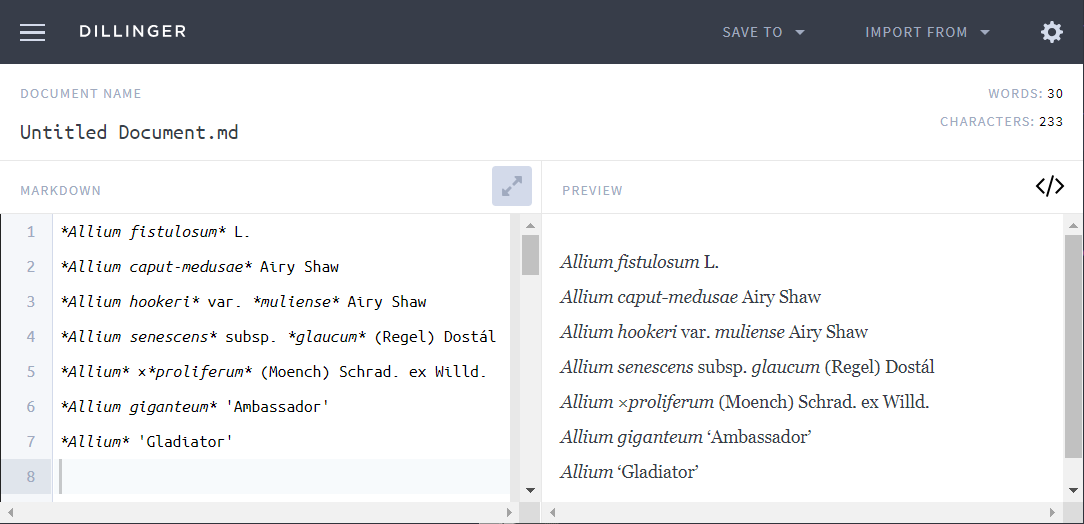
\includegraphics[width=\textwidth]{Illustratio/Markdown_online.png}
\end{frame}


\end{document}
